\documentclass{article}
\usepackage{graphicx}
\graphicspath{ {./images/} }
\title{Assigment 3}
\author{Muthya Narayanachary Akhil (A0229794L)}
\date{February 5, 2024}


\begin{document}
\maketitle

\section*{Question 1}
\subsection*{Part a}

Based on the lecture notes, the boolean expression can be calculated to be the following:
\begin{equation}
    \bar{OUT} = (A + B) \cdot (C \cdot D + E)
\end{equation}

\subsection*{Part b}
The appropriate transistor sizing is the following:

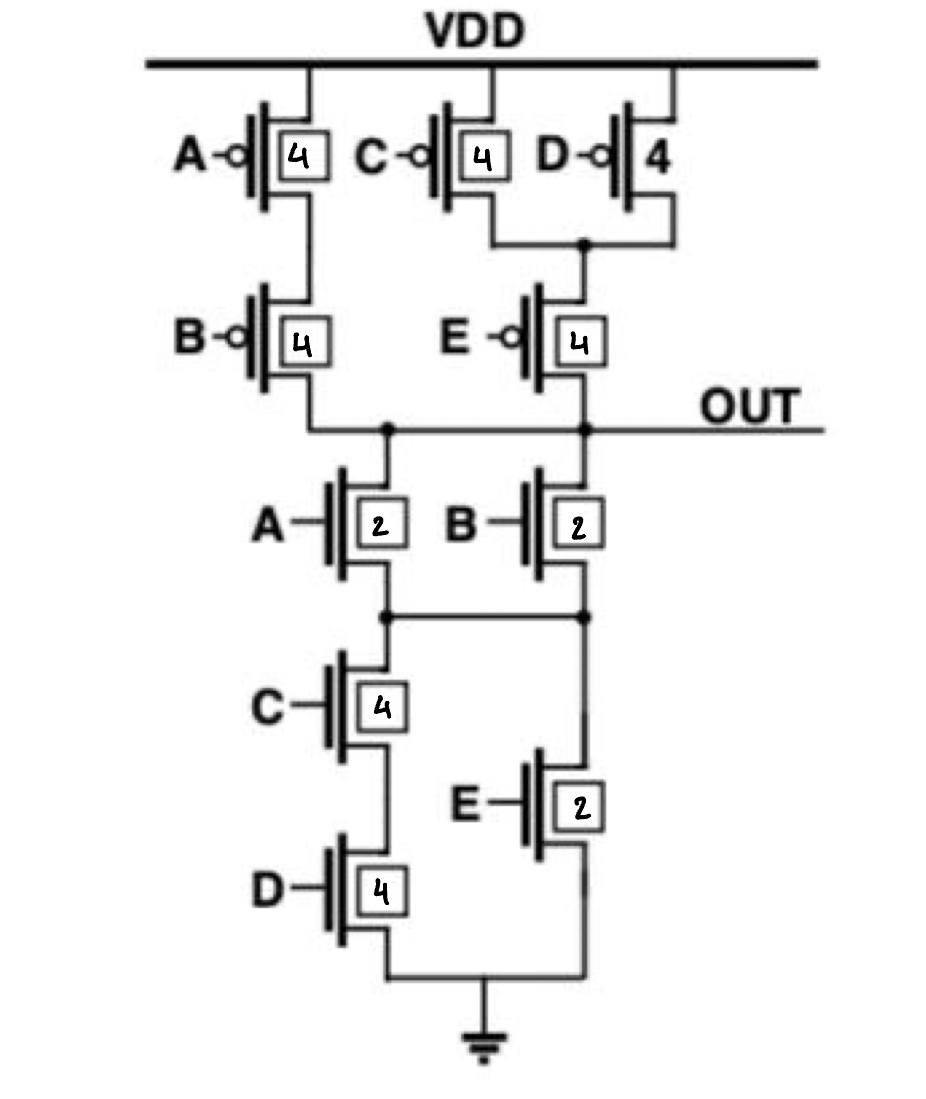
\includegraphics[scale = 0.5]{transistorsizing.png}

\subsection*{Part c}
As discussed in the lecture, the output is low and $R_{out}$ is at its lowest when all the inputs are high
That is:

\begin{equation}
    A = 1,
    B = 1,
    C = 1,
    D = 1,
    E = 1,
\end{equation}

This resistance value is equal to:
\begin{equation}
    R_{out} = \frac{\frac{12k}{2}}{\frac{12k}{2}} + \frac{\frac{12k}{4} + \frac{12k}{4}}{\frac{12k}{2}} = 6k\Omega
\end{equation}

\subsection*{Part d}
Similarly, when the output is high, $R_{out}$ is lowest when all the inputs are low.
That is:

\begin{equation}
    A = 0, B= 0, C = 0, D = 0, E = 0
\end{equation}

And the output resistance can be caculated to be:
\begin{equation}
    R_{out} = \frac{\frac{12k}{2} + \frac{12k}{2}}{\frac{\frac{12k}{2}}{\frac{12k}{2}} + \frac{12k}{2}} = 5.14K\Omega
\end{equation}

\subsection*{Part e}
As seen in the lecture, this can be calcuated in the following manner
\begin{equation}
    t_{pLH, best} = 0.69 * 5.14k * 100f = 355 ps
\end{equation}

\begin{equation}
    t_{pHL, best} = 0.69 * 6k * 100f = 414 ps
\end{equation}

\section*{Question 2}
\subsection*{Part a}
This circuit performs the function of a NAND gate. The PASS transistor network performs AND
then an inverter  by M1 and M2.

\subsection*{Part b}
When A=B=1, the pass transistor would pass up to VDD - $V_{th(NMOS)}$ to the $X^{nth}$ node.
This results in M1 not completely turning off which leads to static power dissipation as both
M1 and M2 are on.

\subsection*{Part c}
This can be done in the following way:

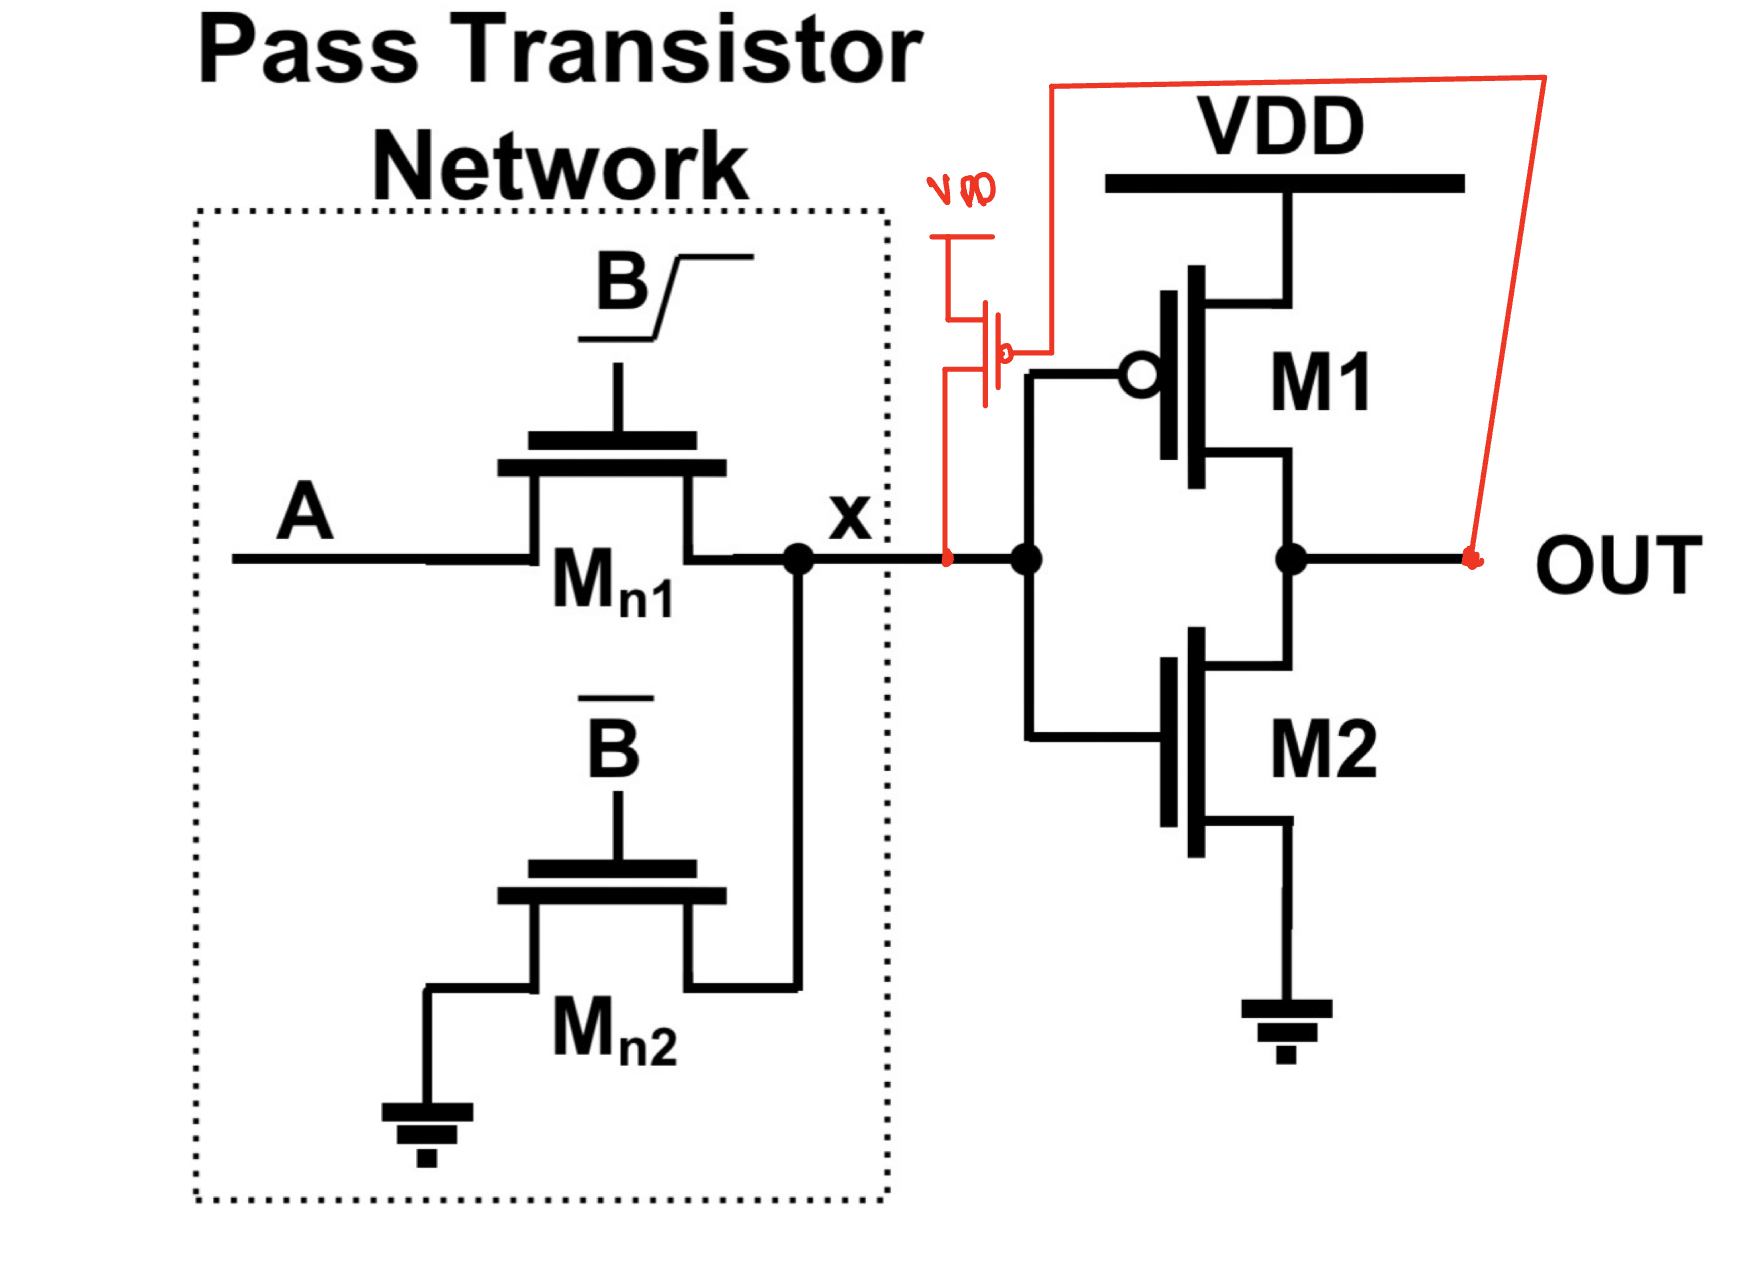
\includegraphics[scale = 0.15]{q2pc.jpeg}

One should note that the transistor should be small enough to pull the node X to GND
when B is 0

\subsection*{Part d}
This can be done in the following way:

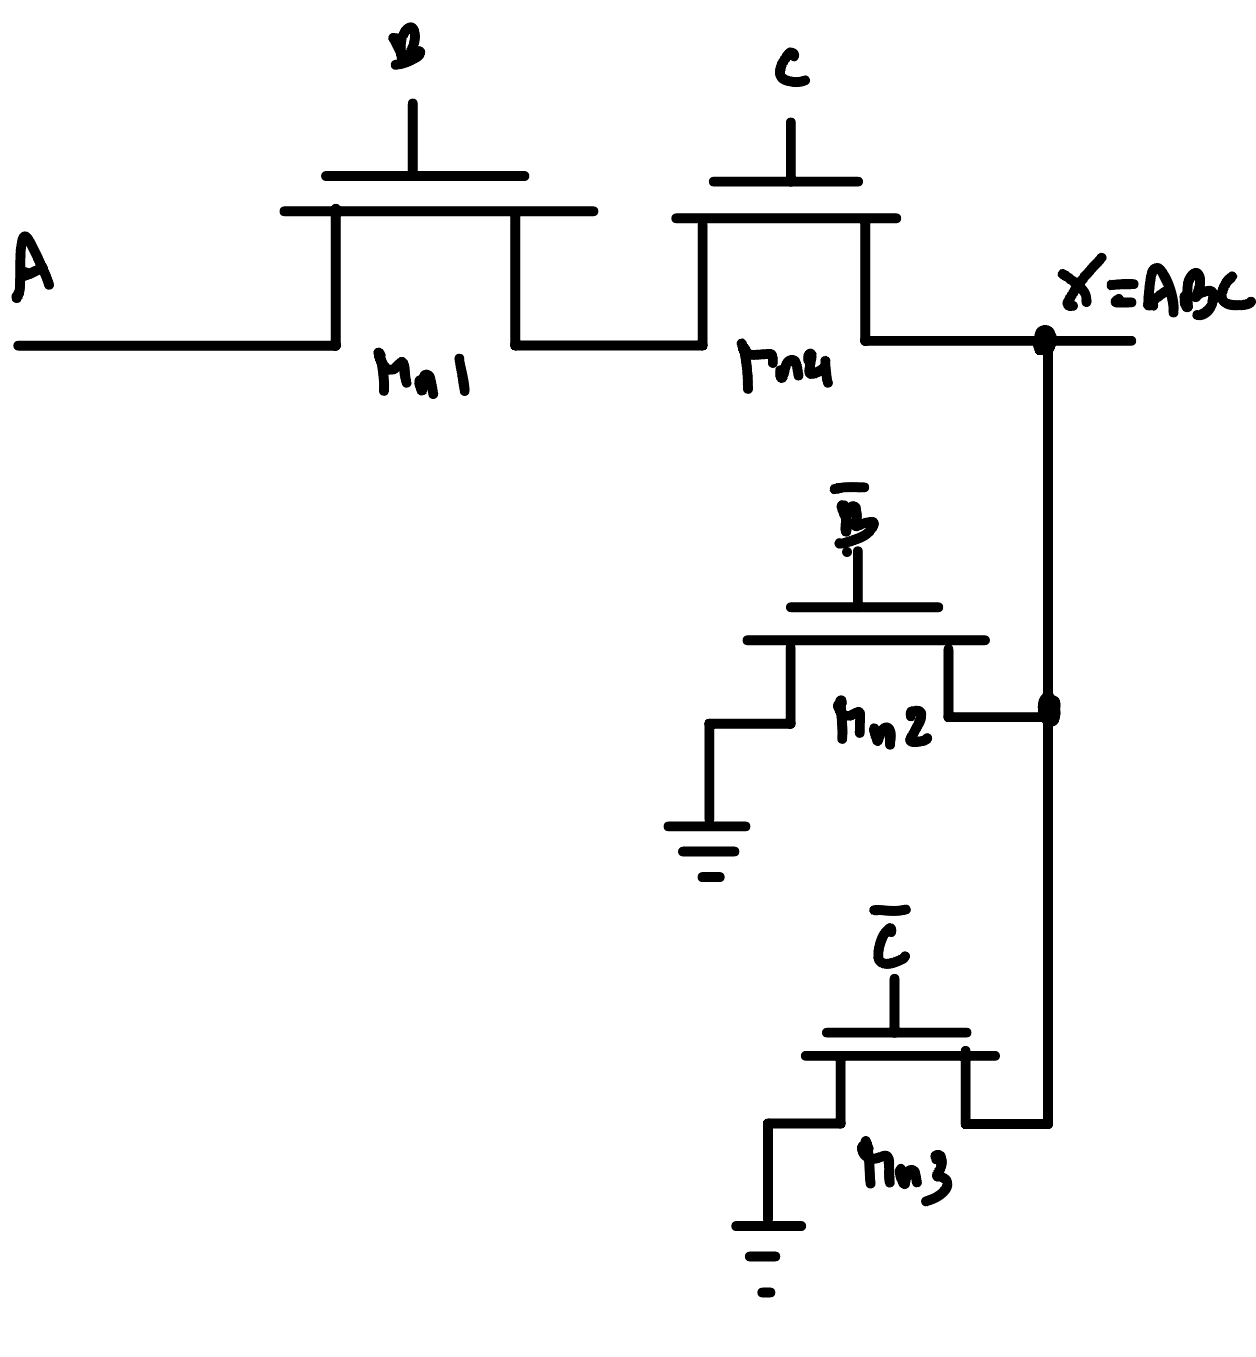
\includegraphics[scale = 0.15]{q2pd.jpeg}

\end{document} 